%%%%%%%%%%%%%%%%%%%%%%%%%%%%% Define Article %%%%%%%%%%%%%%%%%%%%%%%%%%%%%%%%%%
\documentclass{article}
%%%%%%%%%%%%%%%%%%%%%%%%%%%%%%%%%%%%%%%%%%%%%%%%%%%%%%%%%%%%%%%%%%%%%%%%%%%%%%%

%%%%%%%%%%%%%%%%%%%%%%%%%%%%% Using Packages %%%%%%%%%%%%%%%%%%%%%%%%%%%%%%%%%%
\usepackage{geometry}
\usepackage{graphicx}
\usepackage{amssymb}
\usepackage{amsmath}
\usepackage{amsthm}
\usepackage{empheq}
\usepackage{mdframed}
\usepackage{booktabs}
\usepackage{lipsum}
\usepackage{graphicx}
\usepackage{color}
\usepackage{psfrag}
\usepackage{pgfplots}
\usepackage{bm}

%plotting graph
%\usepackage{tikz}
%\usepackage{pgfplot}

%pdfs
\usepackage{pdfpages}
%%%%%%%%%%%%%%%%%%%%%%%%%%%%%%%%%%%%%%%%%%%%%%%%%%%%%%%%%%%%%%%%%%%%%%%%%%%%%%%

% Other Settings

%%%%%%%%%%%%%%%%%%%%%%%%%% Page Setting %%%%%%%%%%%%%%%%%%%%%%%%%%%%%%%%%%%%%%%
\geometry{a4paper}

%%%%%%%%%%%%%%%%%%%%%%%%%% Define some useful colors %%%%%%%%%%%%%%%%%%%%%%%%%%
\definecolor{ocre}{RGB}{243,102,25}
\definecolor{mygray}{RGB}{243,243,244}
\definecolor{deepGreen}{RGB}{26,111,0}
\definecolor{shallowGreen}{RGB}{235,255,255}
\definecolor{deepBlue}{RGB}{61,124,222}
\definecolor{shallowBlue}{RGB}{235,249,255}
%%%%%%%%%%%%%%%%%%%%%%%%%%%%%%%%%%%%%%%%%%%%%%%%%%%%%%%%%%%%%%%%%%%%%%%%%%%%%%%

%%%%%%%%%%%%%%%%%%%%%%%%%% Define an orangebox command %%%%%%%%%%%%%%%%%%%%%%%%
\newcommand\orangebox[1]{\fcolorbox{ocre}{mygray}{\hspace{1em}#1\hspace{1em}}}
%%%%%%%%%%%%%%%%%%%%%%%%%%%%%%%%%%%%%%%%%%%%%%%%%%%%%%%%%%%%%%%%%%%%%%%%%%%%%%%

%%%%%%%%%%%%%%%%%%%%%%%%%%%% English Environments %%%%%%%%%%%%%%%%%%%%%%%%%%%%%
\newtheoremstyle{mytheoremstyle}{3pt}{3pt}{\normalfont}{0cm}{\rmfamily\bfseries}{}{1em}{{\color{black}\thmname{#1}~\thmnumber{#2}}\thmnote{\,--\,#3}}
\newtheoremstyle{myproblemstyle}{3pt}{3pt}{\normalfont}{0cm}{\rmfamily\bfseries}{}{1em}{{\color{black}\thmname{#1}~\thmnumber{#2}}\thmnote{\,--\,#3}}
\theoremstyle{mytheoremstyle}
\newmdtheoremenv[linewidth=1pt,backgroundcolor=shallowGreen,linecolor=deepGreen,leftmargin=0pt,innerleftmargin=20pt,innerrightmargin=20pt,]{theorem}{Theorem}[section]
\theoremstyle{mytheoremstyle}
\newmdtheoremenv[linewidth=1pt,backgroundcolor=shallowBlue,linecolor=deepBlue,leftmargin=0pt,innerleftmargin=20pt,innerrightmargin=20pt,]{definition}{Definition}[section]
\theoremstyle{myproblemstyle}
\newmdtheoremenv[linecolor=black,leftmargin=0pt,innerleftmargin=10pt,innerrightmargin=10pt,]{problem}{Problem}[section]
%%%%%%%%%%%%%%%%%%%%%%%%%%%%%%%%%%%%%%%%%%%%%%%%%%%%%%%%%%%%%%%%%%%%%%%%%%%%%%%

%%%%%%%%%%%%%%%%%%%%%%%%%%%%%%% Plotting Settings %%%%%%%%%%%%%%%%%%%%%%%%%%%%%
\usepgfplotslibrary{colorbrewer}
\pgfplotsset{width=8cm,compat=1.9}
%%%%%%%%%%%%%%%%%%%%%%%%%%%%%%%%%%%%%%%%%%%%%%%%%%%%%%%%%%%%%%%%%%%%%%%%%%%%%%%

%%%%%%%%%%%%%%%%%%%%%%%%%%%%%%% Title & Author %%%%%%%%%%%%%%%%%%%%%%%%%%%%%%%%
\title{Chapter 4.2 Area}
\author{Aarav Yadav}
%%%%%%%%%%%%%%%%%%%%%%%%%%%%%%%%%%%%%%%%%%%%%%%%%%%%%%%%%%%%%%%%%%%%%%%%%%%%%%%

\begin{document}
    \maketitle

    \setcounter{section}{4}
    \setcounter{definition}{3}
    \setcounter{theorem}{1}
    \setcounter{problem}{9}

    \section*{Objectives}
    \begin{itemize}
        \item Use sigma notation to write and evaluate a sum
        \item Understand the concept of area
        \item Approximate the area of a plane region
        \item Find the area of a plane region using limits
    \end{itemize}

    \begin{definition}[Sigma Notation]

        The sum of n terms $ a_{1}, a_{2}, a_{3}, ... ,a_{n} $ is written as: 

        $$ \Sigma_{i=1}^n a_{i} = a_{1} + a_{2} + a_{3} + ... + a_{n} $$

        Where i is the \textbf{index of summation}, $ a_{i} $ is the \textbf{ith term} 
        of the sum, and the \textbf{upper and lower bounds of summation} are n and 1.
        
    \end{definition}

    \begin{problem}[Examples of Sigma Notation]

        The upper and lower bounds must be constant with respect to the index of summation.
        However, the lower bound doesn't have to be 1. Any integer less than or equal to 
        the upper bound is legitimate. 

        \begin{itemize}
            \item $ \Sigma_{i=1}^6 $ \indent $ i $ 
            \item $ \Sigma_{i=0}^5 $ \indent $ (i+1) $
            \item $ \Sigma_{j=3}^7 $ \indent $ j^2  $
            \item $ \Sigma_{j=1}^5 $ \indent $ \frac{1}{\sqrt[]{j}} $
            \item $ \Sigma_{k=1}^n $ \indent $ \frac{1}{n} (k^2+1)  $
            \item $ \Sigma_{i=1}^n $ \indent $ f(x_{i})\Delta x$
        \end{itemize}
    \end{problem}
    
    \newpage

    \begin{theorem}[Summation formulas]
        Provide proofs. 
        \begin{itemize}
            \item $ \Sigma_{i=1}^n c = cn$, c is a constant
            \item $ \Sigma_{i=1}^n i = \frac{n(n+1)}{2}$
            \item $ \Sigma_{i=1}^n i^2 = \frac{n(n+1)(2n+1)}{6}$
            \item $ \Sigma_{i=1}^n i^3 = \frac{n^2(n+1)^2}{4}$
        \end{itemize}
    \end{theorem}

    \begin{problem}[Evaluating a Sum]
        Evaluate $ \Sigma_{i=1}^n \frac{i+1}{n^2} $ for $n = 10, 100, 1000, 10,000$.
    \end{problem}

    \newpage
    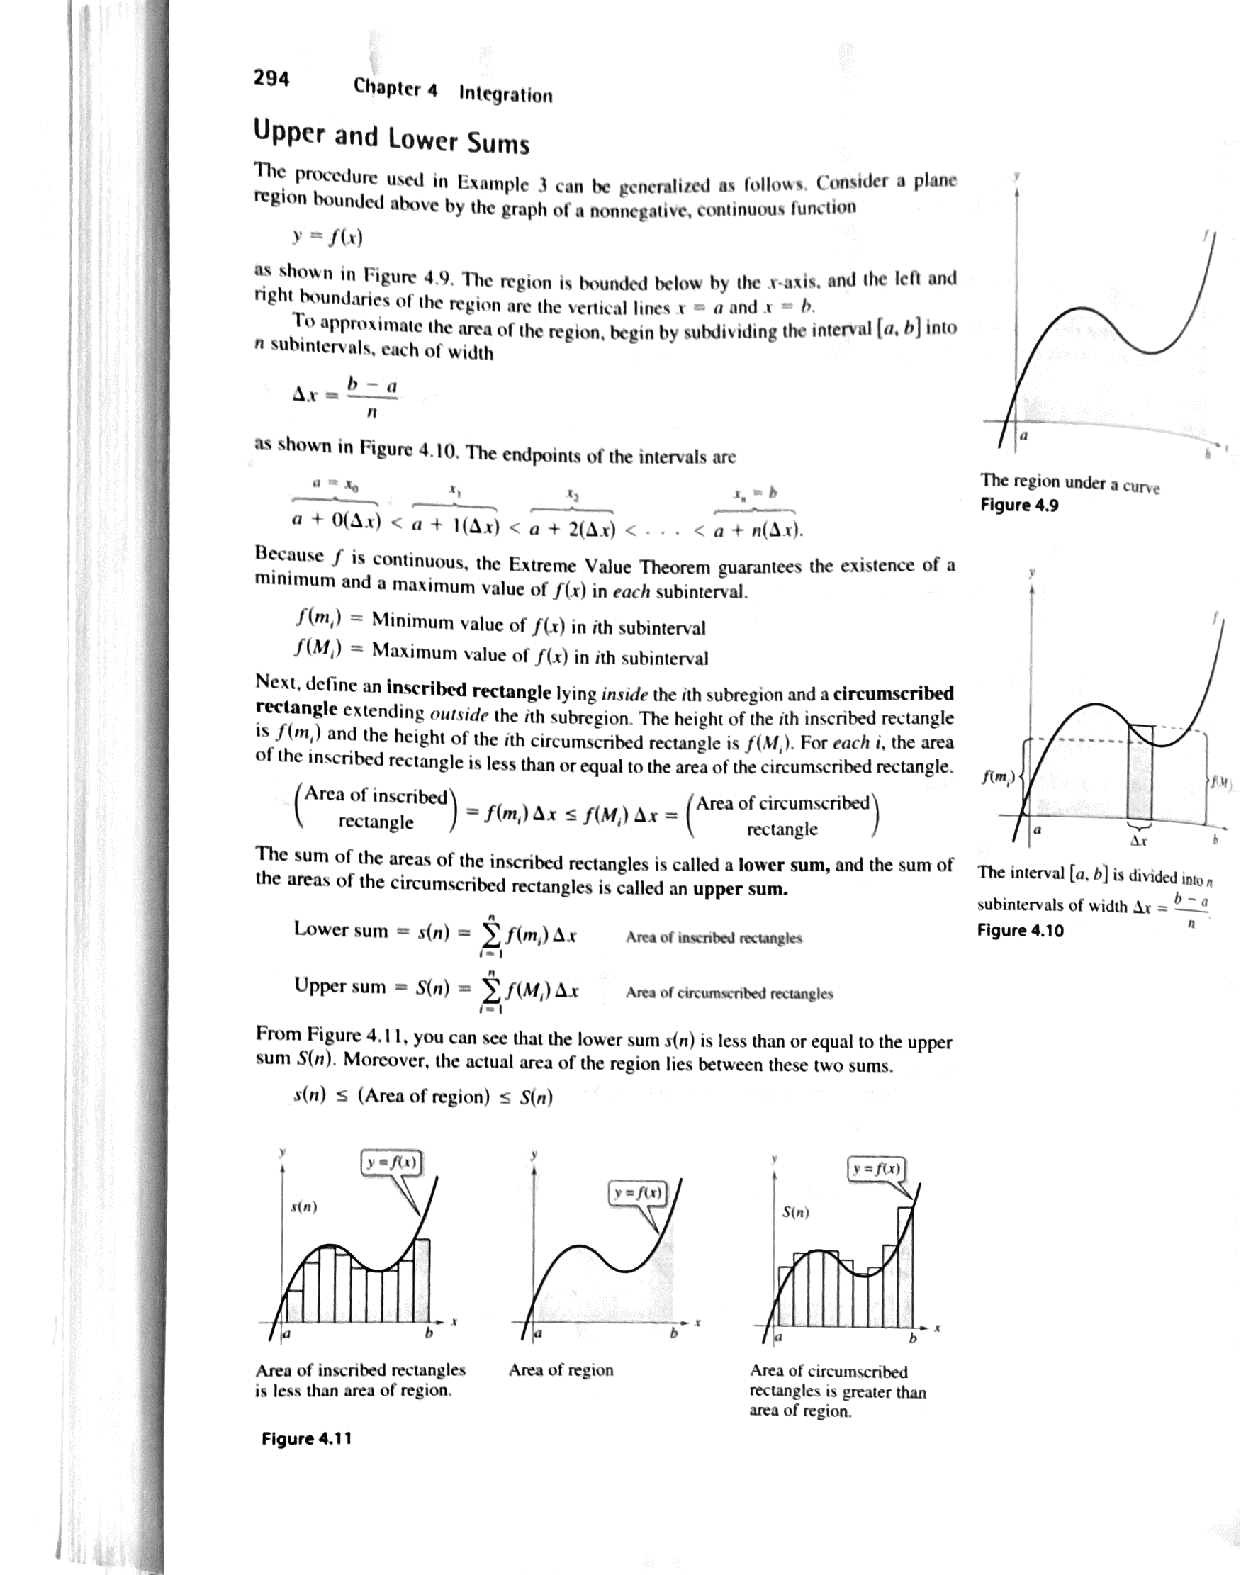
\includepdf[pages=-]{Upper and Lower Sums.pdf}


    \section*{Finding Upper and Lower Sums for a Region Notes}
    Take notes from pg. 294 from textbook.
    \newpage
    

    \begin{problem}[Approximating the Area of a Plane Region]
        Find the upper and lower sums for the region bounded by the graph of $ f(x) = x^2 $
        and the x-axis between x = 0 and x = 2.

        %Plot graph
    \end{problem}

    \begin{problem}[Finding Upper and Lower Sums for a Region]
        Find the upper and lower sums for the region bounded by the graph of 
        $ f(x) = x^2 $ and the x=axis between x = 0 and x = 2. 
    \end{problem}

    \begin{theorem}[Limits of the Lower and Upper Sums]
        Let f be continuous and nonnegative on the interval [a,b]. The limits as
        $ n \rightarrow \infty $ of both the lower and upper sums exist and are equal to
        each other.

        That is,
        $ \lim _{n \to \infty } s(n) = \lim _{n \to \infty } \Sigma_{i=1}^n f(m_{i}\Delta x) $
        
        \indent $ = \lim _{n \to \infty } \Sigma_{i=1}^n f(M_{i}\Delta x) $

        \indent $ = \lim _{n \to \infty } S(n) $
        
        where $\Delta x = (b-a)/n$ and $f(m_{i}) and f(M_{i})$ are the minimum and maximum
        values of f on the subinterval.

    \end{theorem}

    \begin{definition}[Definition of the Area of a Region in the Plane]
        Let f be continuous and nonnegative on the interval [a,b]. The area of the region bounded by the graph
        of f, the x-axis, and the vertical lines x = a and x = b is

        $ Area = \lim _{n \to \infty } \Sigma_{i=1}^n f(c_{i}\Delta x) $

        where, $x_{i-1} <= c_{i} <= x_{i}$ and

        $\Delta x = \frac{b-a}{n}$

        %%PLOT graph
    \end{definition}

    \begin{problem}[Finding Area by the Limit Definition]
        Find the area of the region bounded by the graph $f(x) = x^3$,
        the x-axis, and the vertical lines $x = 0$ and $x = 1$.
    \end{problem}

    \begin{problem}[Finding Area by the Limit Definition]
        Find the area of the region bounded by the graph $f(x) = 4 - x^2$,
        the x-axis, and the vertical lines $x = 1$ and $x = 2$.
    \end{problem}

    \begin{problem}[A Region Bounded by the y-axis]
        Find the area of the region bounded by the graph $f(y) = y^2$,
        the x-axis, and the vertical lines $y = 0$ and $y = 1$.
    \end{problem}

    \begin{problem}[Approximating Area with the Midpoint Rule]
        Use the Midpoint Rule with n = 4 to approximate the area of the region bounded by the graph of 
        $f(x) = sin(x)$ and the x-axis for $0 <= x <= \pi$.
    \end{problem}

\end{document}